\section{Механизм 0-RTT}\label{COMMON.ZeroRTT} 

Располагая согласованным с сервером секретом режима PSK, клиент может начать 
пересылку прикладных данных сразу после отправки 
сообщения~\token[HS.CH]{ClientHello}, не дожидаясь ответа сервера. Данные 
защищаются на общем ключе, который строится по общему секрету. Ранняя отправка 
прикладных данных известна как механизм 0-RTT. Для сравнения, отправка данных 
клиентом после собственного сообщения~\token[HS.F]{Finished} без 
перезапуска Handshake классифицируется как 1-RTT, с перезапуском~---
как 2-RTT.

Клиент сигнализирует о применении механизма 0-RTT, включая
в~\token[HS.CH]{ClientHello} специальное 
расширение~\token[HS.Ext.ed]{early_data}. В 
расширении~\token[HS.Ext.psk]{pre_shared_key} клиент пересылает список 
идентификаторов предварительно согласованных секретов. Ключ механизма 0-RTT
строится по первому секрету этого списка. Сервер объявляет о поддержке
механизма, включая расширение~\token[HS.Ext.ed]{early_data} в свое
сообщение~\token[HS.SH]{ServerHello}.

Пример применения механизма 0-RTT представлен на 
рисунке~\ref{Fig.COMMON.ZeroRTT}. Круглые скобки означают защиту ранних
прикладных данных.

\begin{figure}[hbt]
\begin{center}
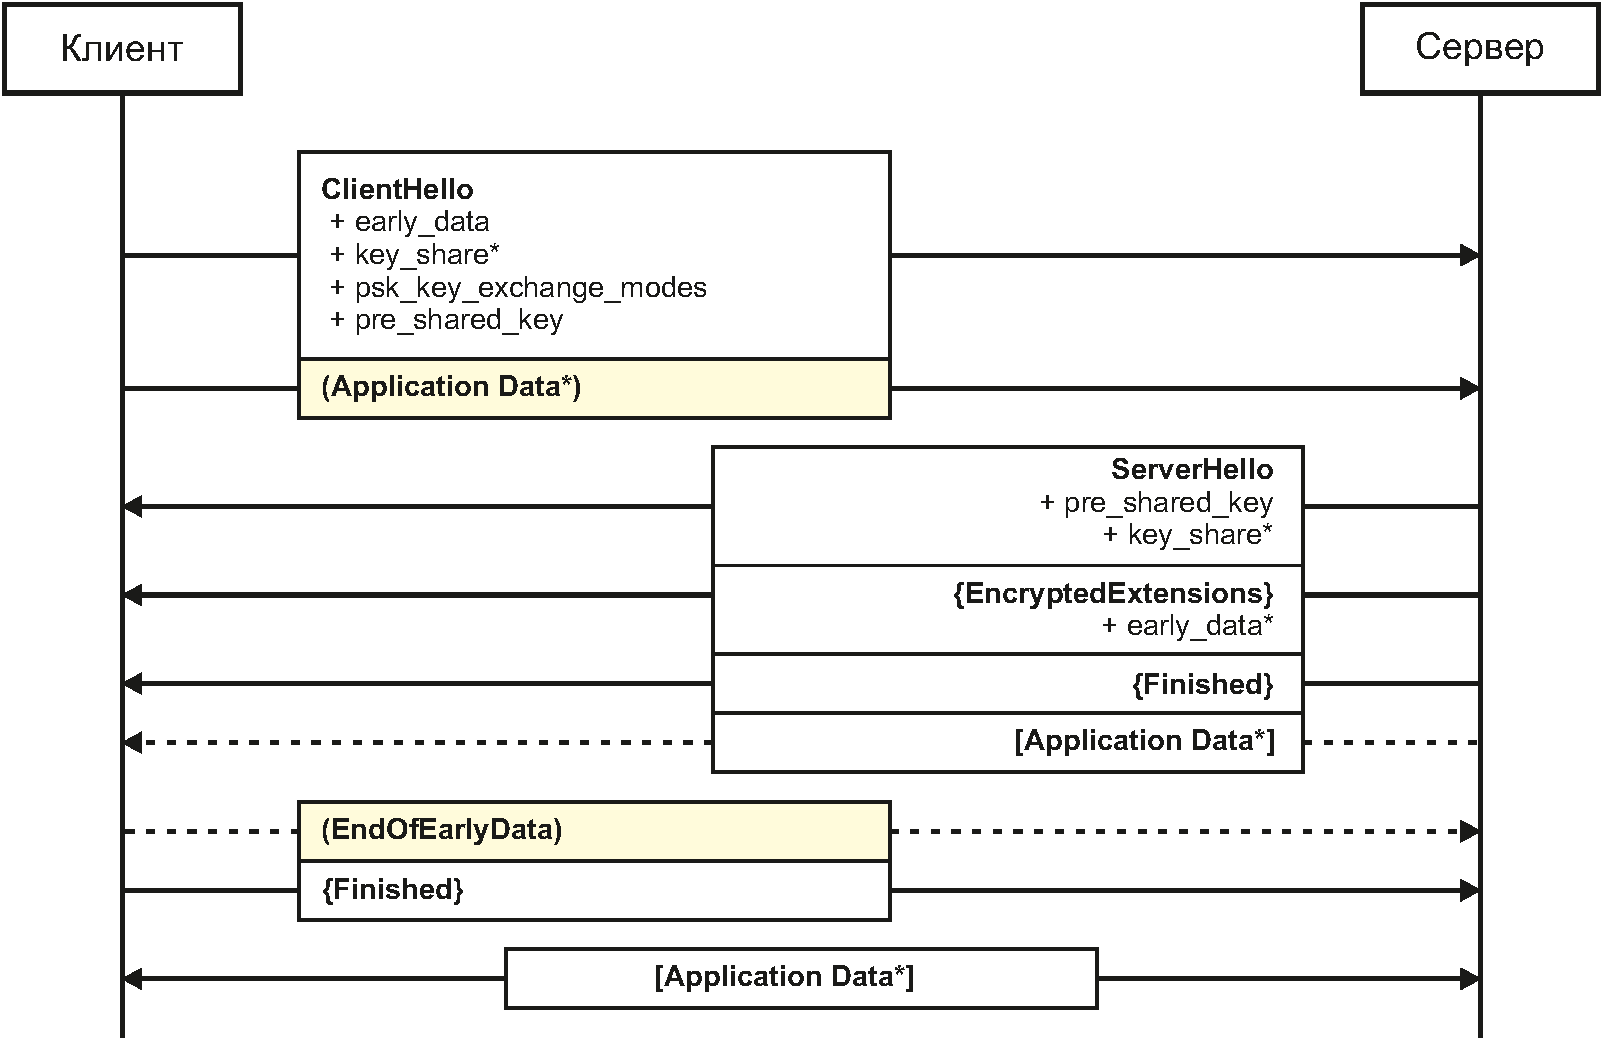
\includegraphics[width=15cm]{../figs/ZeroRTT}
\end{center}
\caption{Механизм 0-RTT}\label{Fig.COMMON.ZeroRTT}
\end{figure}

При планировании использования TLS в прикладных протоколах следует учитывать,
что данные 0-RTT не защищены от <<чтения назад>> и что не обеспечена защита от
повтора этих данных в других соединениях с сервером (эти соединения может
открывать противник без ведома клиента).
%
С другой стороны, данные 0-RTT не могут быть продублированы в текущем
соединении. Более того, противник не может выдать данные 0-RTT за данные 1-RTT 
или 2-RTT, поскольку для защиты используются разные ключи.

% skip: There are no guarantees of non-replay between connections. Protection 
% against replay for ordinary TLS 1.3 1-RTT data is provided via the server's 
% Random value, but 0-RTT data does not depend on the ServerHello and therefore 
% has weaker guarantees. This is especially relevant if the data is 
% authenticated either with TLS client authentication or inside the application 
% protocol. The same warnings apply to any use of the 
% early_exporter_master_secret. 

% skip: Appendix E.5 contains a description of potential attacks, 
% and Section 8 describes mechanisms which the server can use to limit the 
% impact of replay.
